\chapter{Research Methodology}
\label{ch:method}
\sloppy
\hbadness=8000

\section{Overview}
This chapter presents the complete research methodology underpinning the proposed machine learning-based fabric consumption forecasting system. The methodology is structured into six sequential phases: (1)~literature review and problem framing, (2)~physics-informed dataset generation, (3)~data preprocessing and feature engineering, (4)~model training, evaluation, and ensemble construction, (5)~seasonal and fabric-type segmented analysis, and (6)~production deployment via a Streamlit web application. All experiments are designed for full reproducibility using a fixed random seed of 42 throughout. The chapter discusses the research design philosophy, data generation rationale, dataset attributes, preprocessing pipeline, machine learning algorithms, evaluation metrics, training and validation strategy, and application architecture.

\secdiv
\section{Research Design}
This study adopts a quantitative experimental design grounded in the design science research paradigm \cite{hevner2004design}. The design science framework is appropriate because the primary objective is to construct, evaluate, and deploy an artefact---the ML forecasting pipeline---that demonstrably improves upon the existing Bill of Materials (BOM) estimation practice. Quantitative methods enable objective comparison of model performance across standardised metrics (RMSE, MAE, R\textsuperscript{2}, MAPE), while controlled experimental conditions---fixed random seed, identical data splits, and identical preprocessing across all models---ensure that observed performance differences are attributable solely to algorithm design rather than to data partitioning variance.

The six-phase methodology proceeds as follows. Phase~1 surveys the prior literature to identify the research gap and inform feature selection. Phase~2 generates a 5{,}000-order physics-informed synthetic dataset spanning January 2022 to September 2024, capturing the seasonal and garment-type variation typical of an apparel factory's production programme. Phase~3 applies a four-stage preprocessing and feature engineering pipeline to produce clean, encoded, and standardised model inputs. Phase~4 trains four models---Linear Regression (LR), Random Forest (RF), XGBoost, and Long Short-Term Memory (LSTM)---and combines their predictions in a dynamic weighted-average ensemble. Phase~5 performs segmented performance analysis by production season and fabric type to identify where the system is most and least reliable. Phase~6 deploys all trained models within a six-module Streamlit web application designed for direct industrial use.

\secdiv
\section{Proposed System Architecture}

Figure~\ref{fig:architecture} illustrates the end-to-end system architecture, which integrates the data generation module, preprocessing pipeline, four-model training engine, and the Streamlit deployment layer into a single reproducible workflow. Raw order data---including garment type, order quantity, fabric attributes, pattern complexity, and seasonal metadata---flows into the preprocessing module where missing values are handled, categorical features are encoded, and numerical features are standardised. The standardised feature vectors are then passed to each of the four model engines in parallel, after which their predictions are aggregated by the ensemble layer using inverse-RMSE\textsuperscript{2} weighting. The Streamlit application consumes the trained model artefacts (persisted as serialised \texttt{.pkl} and \texttt{.h5} files) and exposes them through six user-facing modules covering single-order predictions, batch processing, ROI analysis, and model performance visualisation. Metadata from each training run is saved to \texttt{model\_metadata.json} to keep the deployment layer synchronised with the latest model weights automatically.

\begin{figure}[htbp]
\centering
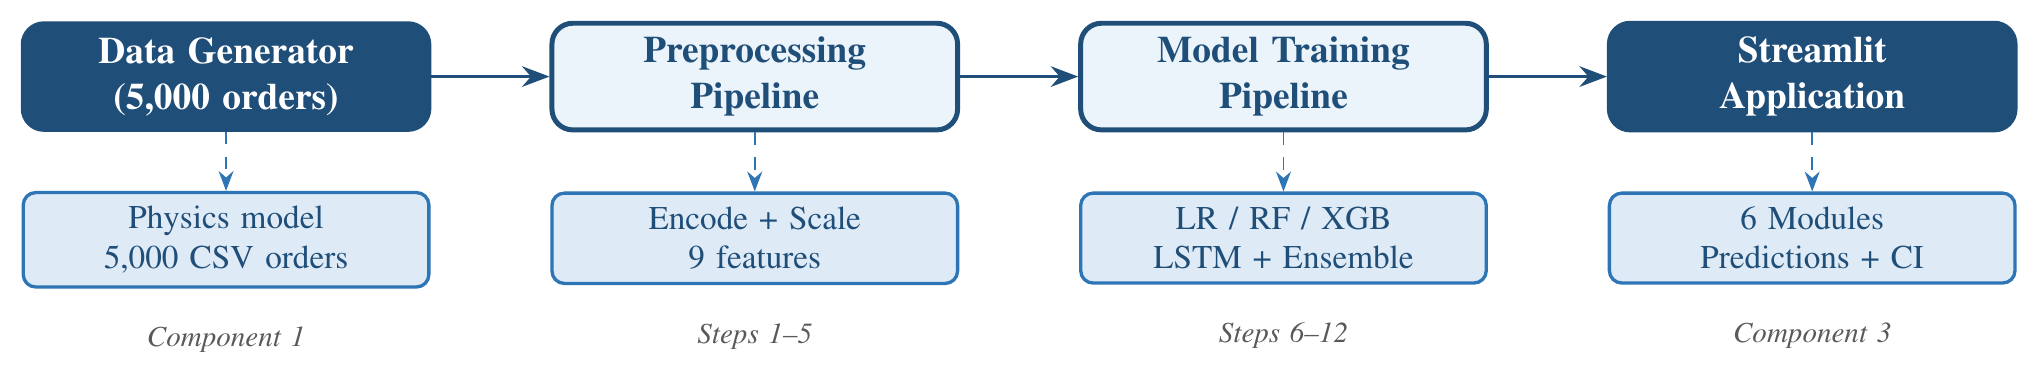
\includegraphics[width=\linewidth]{Chap3/fig_architecture}
\caption{Proposed System Architecture for Material Forecasting}
\label{fig:architecture}
\end{figure}

\secdiv
\section{Research Methodology Flowchart}

Figure~\ref{fig:flowchart} presents the end-to-end research process as a structured flowchart. The flow begins with problem identification and literature-informed dataset design, progresses through the preprocessing and model training stages, and concludes with evaluation, deployment, and impact assessment. Decision nodes at the model evaluation stage support iterative refinement if performance thresholds are not met, ensuring that the deployed system satisfies the study's accuracy and robustness requirements. The flowchart also makes explicit the feedback loop from evaluation back to hyperparameter tuning, which governed the selection of XGBoost's learning rate and tree count and the LSTM's layer sizes and dropout rates.

\begin{figure}[p]
\centering
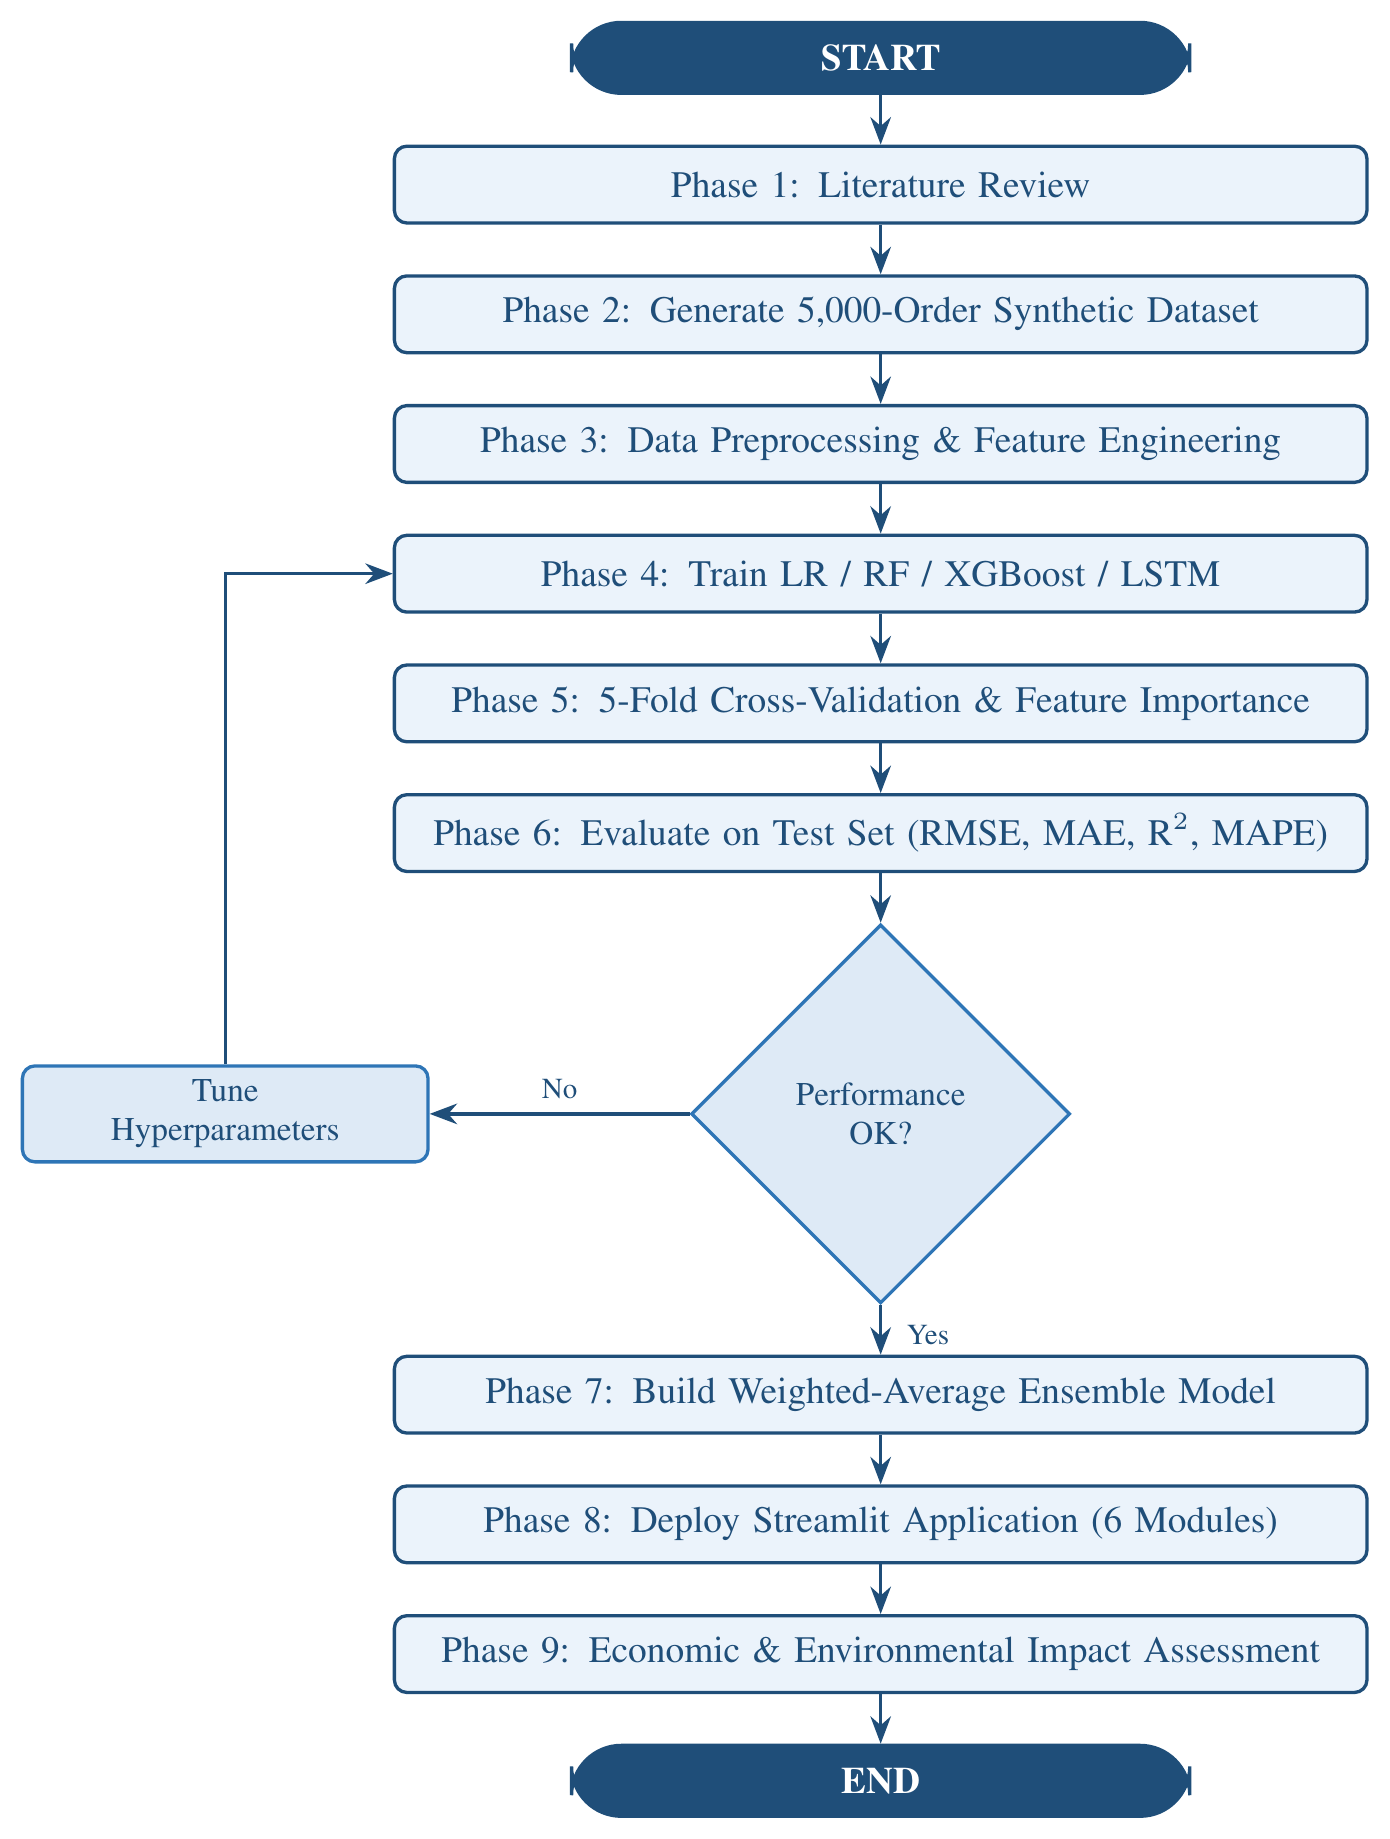
\includegraphics[width=0.72\linewidth]{Chap3/fig_flowchart}
\caption{Research Methodology Flowchart}
\label{fig:flowchart}
\end{figure}

\secdiv
\section{Data Collection and Generation}
\label{sec:datageneration}
Because real factory production records are commercially sensitive and not publicly available at the scale required for rigorous multi-model comparison, a physics-informed synthetic dataset generator was developed in Python. The generator is justified on three grounds. First, \textit{experimental control}: all confounding variables such as supplier fabric batch differences, machine downtime, and seasonal demand shocks are held constant, isolating the deterministic relationship between order attributes and fabric consumption. Second, \textit{reproducibility}: setting \texttt{numpy.random.seed(42)} guarantees that any researcher can regenerate identical datasets, enabling independent verification of all reported metrics. Third, \textit{physical validity}: every generated record satisfies the fundamental fabric consumption equation (Equation~\ref{eq:bom_physics}), augmented with garment-type base coefficients, seasonal weight adjustments, and operator-experience quality factors derived from published apparel engineering literature.

\begin{mdframed}[style=eqbox]
\begin{equation}
\text{Consumption} = \frac{\text{Qty} \times L_{\text{pattern}} \times W_{\text{pattern}}}{W_{\text{fabric}} \times \text{MarkerEff}} \times (1 + \text{DefectRate}) \times \text{Complexity}
\label{eq:bom_physics}
\end{equation}
\end{mdframed}

\noindent The generator produces 5{,}000 production orders covering five garment types (T-Shirt, Shirt, Pants, Dress, Jacket), five fabric categories (Cotton, Polyester, Denim, Silk, Cotton-Blend), four production seasons, and the full range of fabric width and quality parameters observed in mid-scale RMG factories. The generated production dates span January 2022 to September 2024, providing a realistic temporal spread for a mid-scale factory's annual production programme.

\secdiv
\section{Dataset Description}
\label{sec:dataset}
The simulated dataset comprises 34 columns in total; Table~\ref{tab:dataset} describes the 17 ML-pipeline columns, of which 9 serve as ML input features and one---\texttt{Actual\_Cons\_yd}---is the regression target. Table~\ref{tab:dataset} summarises all attributes with their data types, value ranges, and roles in the forecasting model. The nine input features capture three distinct sources of fabric consumption variability: (i)~\textit{order-level scale drivers}---Order\_Qty, Garment\_Type, and Pattern\_Cmplx---which together account for 91.7\% of XGBoost's feature importance; (ii)~\textit{fabric and cut parameters}---Fabric\_Width\_in and Fabric\_Type---which govern marker utilisation and lot-level consumption rates; and (iii)~\textit{production quality factors}---Marker\_Eff\_\%, Defect\_Rate\_\%, Operator\_Exp, and Season---which introduce stochastic variation around the physics baseline. The column \texttt{Planned\_BOM\_yd} records the output of the physics formula (Equation~\ref{eq:bom_physics}) for reference and BOM baseline comparisons, but is deliberately excluded from the nine ML input features to test whether operationally observable attributes alone can match or exceed the physics model's predictive accuracy.

{\scriptsize\tabcolsep=3pt
\begin{longtable}{@{}L{2.8cm} C{1.2cm} L{3.2cm} L{7.2cm}@{}}
  \caption{Simulated Dataset Attributes and Descriptions}
  \label{tab:dataset}\\
  \toprule
  \textbf{Feature}&\textbf{Type}&\textbf{Range / Values}&\textbf{Role \& FI Score}\\
  \midrule\endfirsthead
  \toprule
  \textbf{Feature}&\textbf{Type}&\textbf{Range / Values}&\textbf{Role \& FI Score}\\
  \midrule\endhead\bottomrule\endfoot
  Order\_ID&Nominal&ORD\_0001\ldots&Identifier; not ML input\\
  Order\_Date&Date&Jan 22--Sep 24&Temporal tag\\
  Order\_Qty&Numeric&100--5k units&Key scale driver; FI=0.30\\
  Garment\_Type&Nominal&T-Shirt, Shirt, Pants, Dress, Jacket&Base coeff; FI=0.52\\
  Fabric\_Type&Nominal&Cotton, Poly, Denim, Silk, Blend&Predictability; FI=0.007\\
  Fabric\_W\_in&Numeric&55, 59, 63, 71 in&Width adj.; FI=0.04\\
  Fabric\_W\_cm&Numeric&139.7--180.3cm&Derived: in$\times$2.54\\
  Pattern\_Cmplx&Ordinal&Simple/Med/Comp&Complexity mult.; FI=0.10\\
  Season&Nominal&Spr, Sum, Fall, Win&Seasonal offset; FI=0.007\\
  Marker\_Eff\_\%&Numeric&70--95\%&Waste factor; FI=0.01\\
  Defect\_Rate\_\%&Numeric&0--10\%&Waste amplifier; FI=0.009\\
  Operator\_Exp&Numeric&1--20 yrs&Quality; FI=0.01\\
  Fabric\_GSM&Numeric&100--300&Context only\\
  Planned\_BOM\_yd&Numeric&Continuous&Physics BOM (not in 9-feat set)\\
  \textbf{Actual\_Cons\_yd}&Numeric&Continuous&\textbf{TARGET}\\
  Variance\_yd&Numeric&$-$14.22\% to $+$19.92\%&Actual$-$Planned BOM\\
  Measure\_Unit&String&``yards''&Unit confirmation\\
\end{longtable}
}

\noindent Across the full 5{,}000-order dataset, mean actual fabric consumption is 8{,}288\,yd (SD 5{,}688\,yd), reflecting the broad range of order scales from small bespoke runs of 100 units to high-volume commodity orders of 5{,}000 units. The mean planned BOM is 8{,}449\,yd, indicating a systematic over-planning bias of approximately 1.9\% embedded in the physics formula's 5\% safety buffer. Approximately 42\% of orders over-consume relative to the BOM plan, while BOM-to-actual variance ranges from $-$14.22\% to $+$19.92\% across the full dataset, confirming that the static BOM estimate is insufficient for capturing the full distribution of production outcomes.

\secdiv
\section{Data Preprocessing Pipeline}

Figure~\ref{fig:preprocessing} illustrates the four-stage preprocessing pipeline applied to the raw dataset before any model training. In the \textit{first stage}, a completeness and consistency check verifies that the 5{,}000-order dataset contains no missing values and no attribute values outside physical plausibility bounds. This quality confirmation is a consequence of the controlled generation process and ensures that downstream models are not exposed to imputation artefacts. In the \textit{second stage}, feature engineering derives \texttt{Fabric\_Width\_cm} from \texttt{Fabric\_Width\_in} by multiplying by 2.54, providing a metric-unit equivalent retained alongside the original imperial measure. In the \textit{third stage}, label encoding is applied to the three nominal categorical features (Garment\_Type, Fabric\_Type, Season) and ordinal encoding to Pattern\_Complexity (Complex=0, Medium=1, Simple=2, following alphabetical LabelEncoder ordering). Label encoding is preferred over one-hot encoding for tree-based models because it avoids high-cardinality dimensionality expansion that can slow XGBoost and Random Forest training without improving accuracy \cite{chen2016xgboost}. In the \textit{fourth stage}, all nine numerical input features are standardised using \texttt{sklearn.preprocessing.StandardScaler}, which is fitted exclusively on the training partition and then applied to validation and test sets. This strict fit-on-train-only discipline prevents information leakage that would otherwise produce overly optimistic validation and test metrics.

\begin{figure}[htbp]
\centering
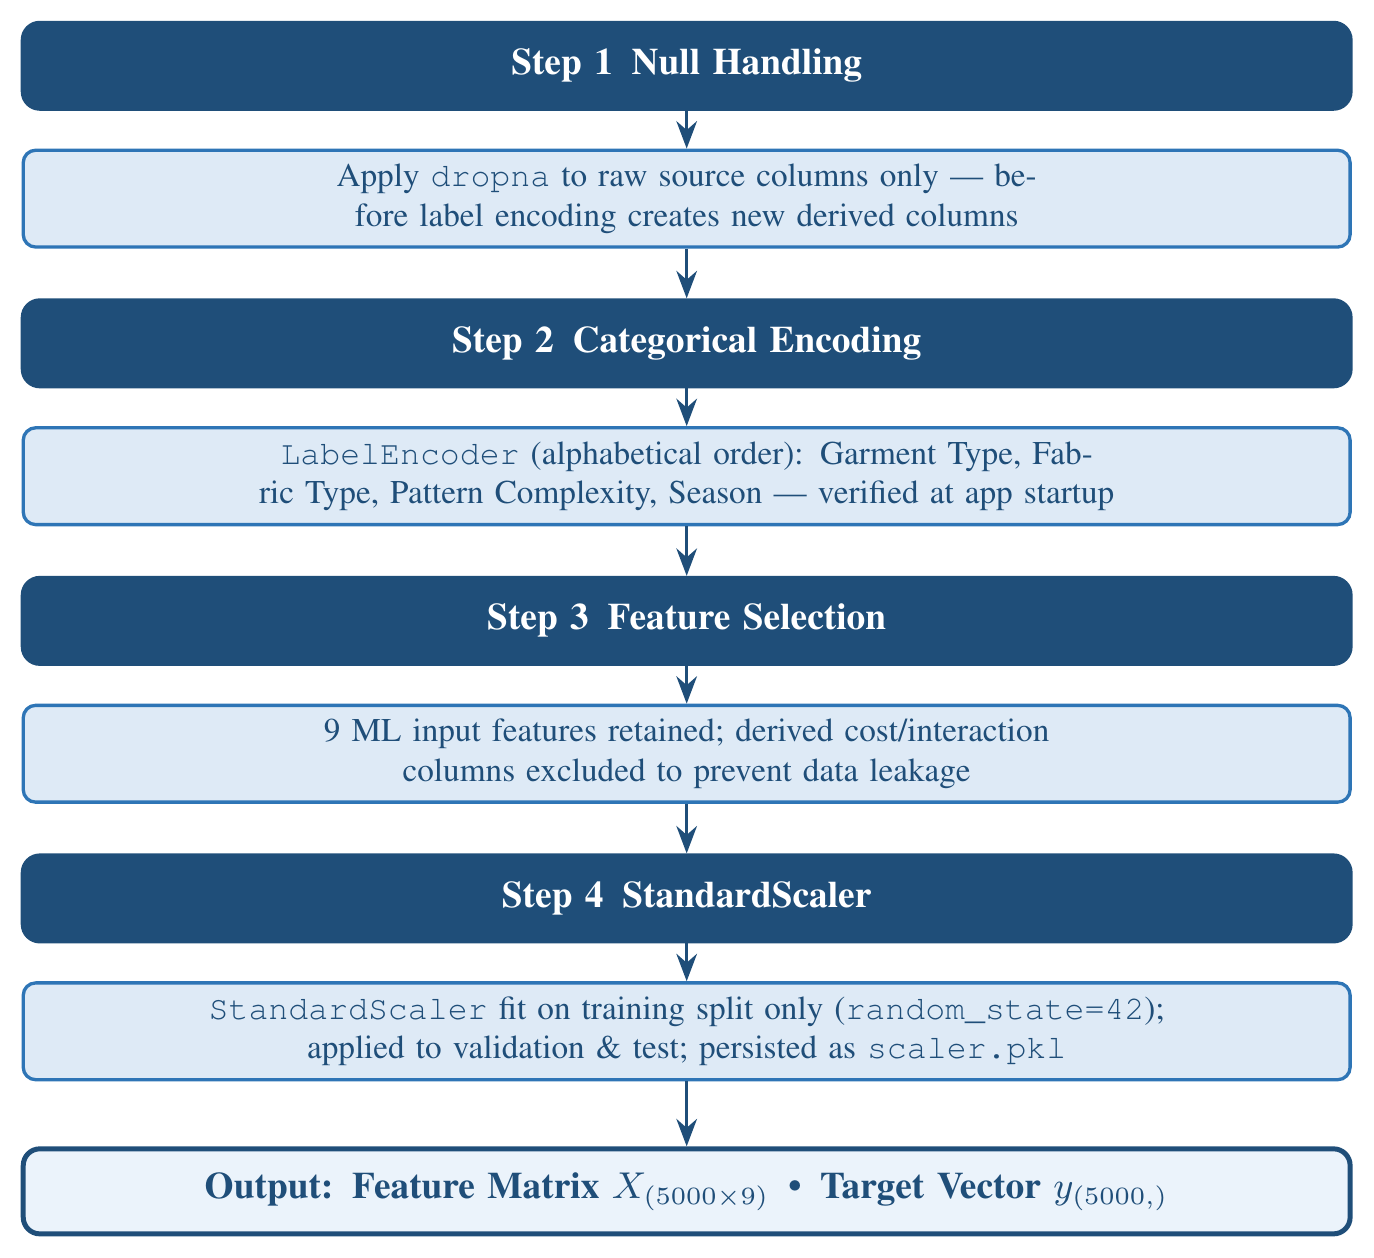
\includegraphics[width=0.78\linewidth]{Chap3/fig_preprocessing}
\caption{Data Preprocessing Pipeline (4 sequential steps)}
\label{fig:preprocessing}
\end{figure}

\secdiv
\section{Feature Engineering}
The preprocessing step constructs two derived features from existing columns. The first, \texttt{Fabric\_Width\_cm}, is computed as $\texttt{Fabric\_Width\_in} \times 2.54$; both width representations are retained as input features to allow models to capture the width value in the unit most relevant to each model's internal representation. The second derived variable, \texttt{Planned\_BOM\_yd}---the output of the physics-formula estimate---is not included in the nine ML input features but is retained as a context column for BOM baseline performance benchmarking. This deliberate exclusion creates a controlled test of whether the nine operationally observable features alone can achieve forecasting accuracy comparable to or exceeding the full physics formula. The LSTM's R\textsuperscript{2}=0.9955 compared to the BOM's R\textsuperscript{2}=0.9927 confirms that they can, providing a margin of improvement that justifies the additional modelling complexity.

\secdiv
\section{Machine Learning Algorithms}

\subsection{Linear Regression}
Linear Regression (LR) is included as an interpretable baseline that represents the simplest possible parametric mapping from input features to fabric consumption. It fits a linear combination of the nine standardised features to minimise the sum of squared residuals, as expressed in Equation~\ref{eq:lr}. While computationally efficient (training time $\approx$0.8\,s), LR cannot capture the multiplicative interaction between garment type and order quantity that drives the non-linear consumption curve. Its inclusion in the study serves to quantify the performance gap attributable to model non-linearity.

\begin{mdframed}[style=eqbox]
\begin{equation}\hat{y}=\beta_0+\sum_{j=1}^{9}\beta_j x_j\label{eq:lr}\end{equation}
\end{mdframed}

\subsection{Random Forest}
Random Forest (RF) constructs an ensemble of $B=300$ decorrelated decision trees, each trained on a bootstrapped sample of the training data, and averages their predictions as shown in Equation~\ref{eq:rf}. The bootstrap aggregation mechanism reduces variance by averaging out the individual trees' overfitting tendencies, while the random feature subsampling at each split ensures that trees are sufficiently different to provide diverse error correction. RF is selected because it handles non-linear relationships and feature interactions without requiring explicit polynomial terms, while remaining computationally manageable and robust to irrelevant features.

\begin{mdframed}[style=eqbox]
\begin{equation}\hat{y}_{\text{RF}}(\mathbf{x})=\frac{1}{B}\sum_{b=1}^{B}T_b(\mathbf{x}),\quad B=300\label{eq:rf}\end{equation}
\end{mdframed}

\subsection{XGBoost}
XGBoost implements gradient-boosted decision trees with a learning rate $\eta=0.08$, 300 estimators, and $L_1$/$L_2$ regularisation terms $\alpha$ and $\lambda$ (Equation~\ref{eq:xgb}). Each successive tree $h_m$ is fitted to the negative gradient of the loss function, progressively correcting the residual errors of all prior trees. The regularisation penalty $\Omega$ prevents the deep ensemble from memorising training data, contributing to strong generalisation on the held-out test set. XGBoost is chosen as the primary tree-based model over Random Forest because its sequential boosting strategy is better suited to progressively reducing the structured non-linear residuals that arise from the garment-type$\times$order-quantity interaction. Crucially, XGBoost also provides gain-based feature importance scores that are used in Section~\ref{sec:fi} to identify the dominant predictors of fabric consumption and guide data quality investment priorities.

\begin{figure}[htbp]
\centering
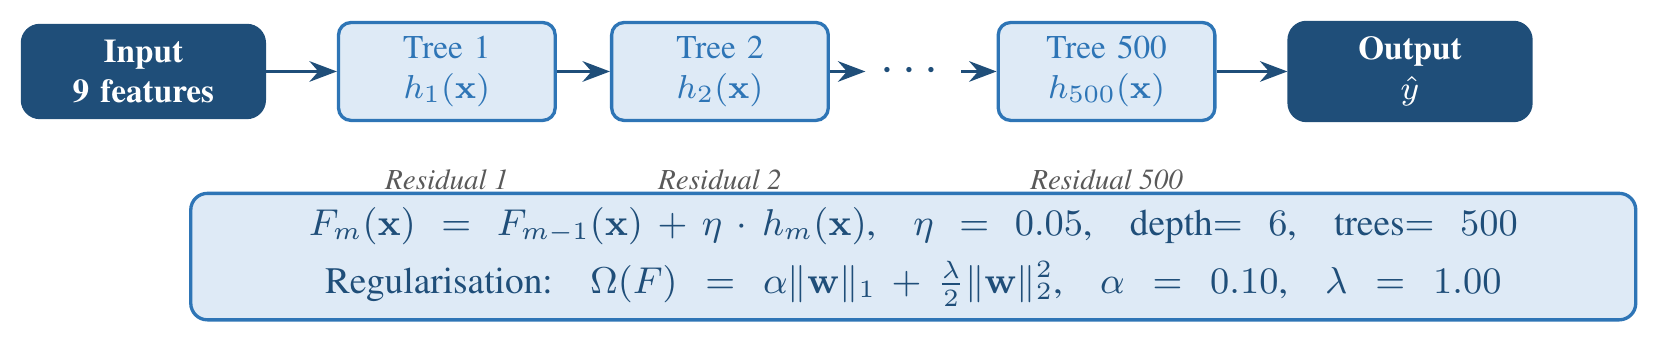
\includegraphics[width=\linewidth]{Chap3/fig_xgboost}
\caption[XGBoost Architecture]{XGBoost Gradient Boosting Architecture (300 sequential trees, $\eta$=0.08)}
\label{fig:xgboost}
\end{figure}

\begin{mdframed}[style=eqbox]
\begin{equation}F_m(\mathbf{x})=F_{m-1}(\mathbf{x})+\eta\cdot h_m(\mathbf{x}),\quad\Omega=\alpha\|\mathbf{w}\|_1+\tfrac{\lambda}{2}\|\mathbf{w}\|_2^2\label{eq:xgb}\end{equation}
\end{mdframed}

\subsection{LSTM Neural Network}
The Long Short-Term Memory (LSTM) network is a recurrent architecture originally designed for sequential time-series data. In this study it is adapted as a high-capacity non-linear function approximator for tabular production-order data, exploiting its ability to model higher-order feature interactions through recurrent hidden states. The architecture follows a stacked LSTM design: the 9-feature input vector is reshaped to a $(n, 1, 9)$ three-dimensional tensor and passed through two LSTM layers (64 units, then 32 units), each followed by a Dropout layer (rate=0.2) for regularisation, before terminating in a Dense(16, ReLU) hidden layer and a scalar Dense(1) output layer. The network is trained with the Adam optimiser ($\eta$=0.001), mean-squared-error loss function, a mini-batch size of 32, a maximum of 200 epochs, an early-stopping callback (patience=15) monitoring validation loss to prevent overfitting, and a learning-rate scheduler (ReduceLROnPlateau: factor=0.5, patience=6) that halves the Adam learning rate whenever validation loss plateaus for six consecutive epochs, enabling finer convergence in later training stages. The two-layer stacked architecture captures higher-order non-linear interactions---particularly the multiplicative garment$\times$quantity$\times$complexity relationship---that tree-based models approximate only coarsely through piecewise constant decision boundaries.

\secdiv
\section{Model Evaluation Metrics}
\label{sec:metrics}
Four complementary metrics are used to evaluate and compare model performance, as formally defined in Equations~\ref{eq:m1}--\ref{eq:m2}.

\begin{mdframed}[style=eqbox]
\begin{align}
\text{RMSE}&=\sqrt{\tfrac{1}{n}\sum(y_i-\hat{y}_i)^2}&\text{MAE}&=\tfrac{1}{n}\sum|y_i-\hat{y}_i|\label{eq:m1}\\
R^2&=1-\tfrac{\sum(y_i-\hat{y}_i)^2}{\sum(y_i-\bar{y})^2}&\text{MAPE}&=\tfrac{100}{n}\sum\tfrac{|y_i-\hat{y}_i|}{y_i}\label{eq:m2}
\end{align}
\end{mdframed}

\noindent Root Mean Squared Error (RMSE) is adopted as the primary metric because it penalises large errors quadratically---a property directly aligned with the procurement objective of minimising costly over- or under-ordering events. Mean Absolute Error (MAE) provides a robust, outlier-insensitive average error in interpretable units of yards, making it easily communicated to non-technical procurement managers. The coefficient of determination R\textsuperscript{2} quantifies the proportion of variance in actual consumption explained by the model, with values approaching 1.0 indicating near-perfect fit. Mean Absolute Percentage Error (MAPE) provides a scale-independent view that enables comparison across orders of widely differing sizes, although it must be interpreted with caution for very small denominators (low-consumption orders) where percentage errors can be disproportionately large.

\secdiv
\section{Training and Validation Strategy}
\label{sec:strategy}
The 5{,}000-order dataset is partitioned into training (64\%, 3{,}200 orders), validation (16\%, 800 orders), and test (20\%, 1{,}000 orders) subsets using random sampling with seed=42 (Table~\ref{tab:split}). The training set is used exclusively for model weight and parameter fitting. The validation set guides hyperparameter selection and, for the LSTM, provides the early-stopping signal to terminate training before overfitting sets in. The test set is held completely separate throughout the entire development cycle---it is not used for any tuning decision---and is used only once for final reported performance metrics, providing an unbiased estimate of how each model will perform on genuinely new production data.

\begin{table}[htbp]
\centering\caption{Train-Validation-Test Split Configuration}\label{tab:split}
\begin{tabularx}{\textwidth}{@{}L{3cm} C{2.5cm} C{2.5cm} X@{}}
  \toprule\rowcolor{tableheadbg}\tblhdr{Split}&\tblhdr{Proportion}&\tblhdr{Rows}&\tblhdr{Purpose}\\
  \midrule
  Training&64\%&3{,}200&Weight fitting\\
  Validation&16\%&800&Tuning; early stop\\
  Test&20\%&1{,}000&Final evaluation\\
  \bottomrule
\end{tabularx}
\end{table}

Five-fold cross-validation is performed on the combined training-plus-validation partition (4{,}000 orders) for the three classical models to assess whether test-set performance is representative of performance on different random data partitions. The test set is strictly excluded from cross-validation to avoid information leakage. LSTM is excluded from cross-validation due to its prohibitive training cost ($\approx$33\,s per fold $\times$ 5 = $\approx$2.75 minutes) and the sensitivity of stochastic gradient descent convergence to fold-level initialisation conditions.

The weighted-average ensemble combines the four base models' predictions using dynamic inverse-RMSE\textsuperscript{2} weights (Equation~\ref{eq:ens}). This weighting scheme assigns each model a weight proportional to the reciprocal of the square of its validation-set RMSE, automatically giving higher influence to models with lower prediction error. The squared reciprocal formulation exaggerates the weight differential compared to simple inverse-RMSE, making the ensemble more decisive in favouring accurate models. This scheme is fully adaptive: if a base model improves after retraining, its weight increases proportionally without any manual recalibration.

\begin{mdframed}[style=eqbox]
\begin{equation}\hat{y}_{\text{ens}}=\sum_{k}w_k\hat{y}_k,\quad w_k=\frac{1/\text{RMSE}_k^2}{\sum_j 1/\text{RMSE}_j^2}\label{eq:ens}\end{equation}
\end{mdframed}

\secdiv
\section{Application Design}
The trained models are deployed as a production-ready web application built with Streamlit, a Python-native framework that creates interactive data applications without requiring front-end development expertise. Table~\ref{tab:app} summarises the six application modules and their user benefits.

The \textit{Dashboard} module displays key performance indicators (KPIs) including mean RMSE and MAPE, cost savings estimates, and trend charts showing predicted vs.\ actual consumption across the test set. The \textit{Single Prediction} module provides a form-based interface where a planner enters order attributes and receives an instantaneous fabric consumption prediction accompanied by a 90\% confidence interval and a comparison to the BOM estimate. The \textit{Batch Prediction} module accepts a CSV upload of multiple orders and returns a downloadable results file with ML predictions for all rows, enabling seasonal production programme forecasting before fabric procurement commitments are made. The \textit{ROI Calculator} module computes payback period, five-year net present value, and annual waste-cost reduction given user-specified fabric price and order volume assumptions, supporting management-level business case preparation. The \textit{Performance} module visualises RMSE and MAPE comparisons across all models, cross-validation stability results, and the XGBoost feature importance chart, providing model transparency for technical stakeholders and auditors. The \textit{Documentation} module offers a step-by-step user guide and FAQ to lower the adoption barrier for procurement planners unfamiliar with machine learning outputs.

\begin{table}[htbp]
\centering\caption{Streamlit Application Module Summary}\label{tab:app}
\begin{tabularx}{\textwidth}{@{}L{3.5cm} L{6.5cm} Z@{}}
  \toprule\rowcolor{tableheadbg}\tblhdr{Module}&\tblhdr{Key Features}&\tblhdr{User Benefit}\\
  \midrule
  Dashboard&KPI metrics, trend charts&Operational overview\\
  Single Prediction&Interactive form, CI, BOM comparison&Per-order accuracy\\
  Batch Prediction&CSV upload, bulk inference, download&Production-scale planning\\
  ROI Calculator&Payback, 5-yr NPV, waste reduction&Business case\\
  Performance&RMSE/MAPE charts, CV, feature import.&Model transparency\\
  Documentation&User guide, FAQ&Planner support\\
  \bottomrule
\end{tabularx}
\end{table}

\secdiv
\section{Summary}
This chapter has outlined the comprehensive methodology for the ML-based fabric consumption forecasting system. A physics-informed synthetic dataset of 5{,}000 production orders was designed to provide controlled, reproducible experimental conditions grounded in apparel engineering principles. Four machine learning models---Linear Regression, Random Forest, XGBoost, and LSTM---were selected to span the full spectrum from interpretable linear baselines to high-capacity deep learning architectures, enabling a meaningful comparison of their respective strengths and limitations. A four-stage preprocessing pipeline, a 64/16/20 train-validation-test split, 5-fold cross-validation on the non-test data partition, and dynamic inverse-RMSE\textsuperscript{2} ensemble weighting together ensure rigorous, leakage-free evaluation. The methodology is fully reproducible with random seed~42 and culminates in a production-ready six-module Streamlit application. The experimental results obtained from this methodology are presented and analysed in the following chapter.
